%%% File encoding: UTF-8 äöüÄÖÜß  <-- no German umlauts here? Use an UTF-8 compatible editor!

%%% Magic comments for setting the correct parameters in compatible IDEs
% !TeX encoding = utf8
% !TeX program = pdflatex 
% !TeX spellcheck = de_DE
% !BIB program = biber

\documentclass[bachelor,english,smartquotes]{hgbthesis}

% Valid options in [..]: 
%    Type of work: 'diploma', 'master' (default), 'bachelor', 'internship' 
%    Main language: 'german' (default), 'english'
%    Turn on smart quote handling: 'smartquotes'
%    APA bibliography style: 'apa'
%%%-----------------------------------------------------------------------------

\RequirePackage[utf8]{inputenc} % Remove when using lualatex or xelatex!


% Custom imported packages
\usepackage[bottom]{footmisc}
\usepackage{fancyvrb}
\usepackage{pgf-umlsd}

\graphicspath{{images/}}  % Location of images and graphics
\logofile{logo}           % Logo file: images/logo.pdf (no logo: \logofile{})
\bibliography{references} % Biblatex bibliography file (references.bib)

\definecolor{darkgreen}{rgb}{0.0, 0.5, 0.0}

%%%-----------------------------------------------------------------------------
% Title page entries
%%%-----------------------------------------------------------------------------

\title{Service-to-service Authentication in a Microservice Deployment}
\author{Benjamin Ellmer}
\programname{Mobile Computing}

\programtype{Fachhochschul-Bachelorstudiengang} % select/edit
% \programtype{Fachhochschul-Masterstudiengang}

\placeofstudy{Hagenberg}
\dateofsubmission{2022}{03}{28} % {YYYY}{MM}{DD}

\advisor{FH-Prof. DI Dr. Marc Kurz} % optional

%\strictlicense % restrictive license instead of Creative Commons (discouraged!)

%%%-----------------------------------------------------------------------------
\begin{document}
%%%-----------------------------------------------------------------------------

%%%-----------------------------------------------------------------------------
\frontmatter                                   % Front part (roman page numbers)
%%%-----------------------------------------------------------------------------

\maketitle
\tableofcontents
%\include{front/preface} % A preface is optional
\chapter{Abstract}
The microservice architecture is a currently emerging pattern in software engineering.
Instead of having one huge application, the logic is split into numerous smaller units that fulfill one single purpose.
Therefore function calls within the application migrate to remote calls over the network.
The remote calls between the services have to provide confidentiality, integrity, and authentication.
The Transport Layer Security (TLS) protocol provides confidentiality integrity and authenticates the server to the client, but not the client to the server.
Therefore additional mechanisms are necessary for the mutual authentication of the services.

The most popular service-to-service authentication mechanisms are self-signed JSON Web Tokens (JWT) and mutual TLS (mTLS).
Mutual TLS is an adaptation of the TLS protocol that provides a simple and efficient implementation of service-to-service authentication.
On the other hand, it has few configuration possibilities making it hard to adapt the mechanisms for purposes other than service-to-service authentication.
Self-signed JWTs provide the possibility to embed additional parameters within the JWTs, allowing to adapt the authentication mechanisms to simplify tasks like sharing the end-user context.
Additionally, self-signed JWTs have the significant advantage over mTLS that they allow achieving nonrepudiation by storing the received JWTs and requests.

In the end, it is not valid to say that one authentication mechanism is superior in each situation.
Self-signed JWTs are the preferred authentication mechanism when nonrepudiation is required or when the application shares the end-user context.
mTLS is the preferred authentication mechanism when the aim is to implement service-to-service authentication as simply as possible.
Nevertheless, this does not mean that mTLS is must not be used for complex applications or that self-signed JWTs are inappropriate for simple applications.
		
\chapter{Kurzfassung}

\begin{german}
	Die Microservice Architektur ist ein aufstrebendes Pattern in der Softwareentwicklung.
	Eine Applikation welche anhand der Microservice Architektur aufgebaut ist, besteht aus vielen kleinen Services, die genau einen Zweck erfüllen, anstatt aus einer riesigen Komponente.
	Die verschiedenen Services müssen miteinander kommunizieren, um die Logik der anderen Services zu nutzen.
	Somit werden Funktionsaufrufe innerhalb der Applikation zu Funktionsaufrufen über das Netzwerk.
	Diese Netzwerkkommunikation muss Vertraulichkeit, Integrität und Authentisierung gewährleisten.
	Durch die Verwendung des Transport Layer Security (TLS) Protokolls werden Integrität und Vertraulichkeit gewährleistet.
	Außerdem wird anhand des TLS Protokolls der Server gegenüber dem Client authentisiert, jedoch der Client nicht gegenüber dem Server.
	Hierfür werden zusätzliche Authentisierungsmechanismen benötigt.

	Die verbreitetsten Service-zu-Service Authentisierungsmechanismen sind self-signed JSON Web Tokens (JWT) und mutual TLS (mTLS).
	Mutual TLS ist eine Adaptierung des TLS Protokolls und ermöglicht eine effiziente und einfache Implmentierung von Service-zu-Service Authentisierung.
	Andererseits hat man bei mTLS nur wenig Adaptierungsmöglichkeiten, somit ist es schwer für andere Zwecke anpassbar.
	Self-signed JWTs ermöglichen es zusätzliche Parameter in die JWTs zu integrieren.
	Somit kann der Authentisierungsmechanismus so angepasst werden, dass weitere Aufgaben wie das Weitergeben des End-User Contexts vereinfacht werden.
	Zusätzlich haben self-signed JWTs gegenüber mTLS den Vorteil, dass nonrepudiation (Nichtabstreitbarkeit) gewährleistet werden kann, indem die erhaltenen Requests und JWTs gespeichert werden.

	Schlussendlich kann man nicht sagen, dass einer der beiden Authentisierungsmechanismen in jedem Fall dem anderem gegenüber überlegen ist.
	Self-signed JWTs sind der bevorzugte Authentisierungsmechanismus, wenn nonrepudiation eine Anforderung ist, oder wenn die Applikation dazu neigt den End-User Context zu benötigen.
	mTLS ist der bevorzugte Authentisierungsmechanismus, wenn das Ziel ist, so einfach wie möglich Service-zu-Service Authentisierung zu implementieren.
	Trotzdem man nicht sagen kann, dass man mTLS nicht für komplexe Anwendungsfälle geeignet ist, oder dass self-signed JWTs nicht für einfachere Anwendungsfälle geeignet sind.
\end{german}
			

%%%-----------------------------------------------------------------------------
\mainmatter                                    % Main part (arabic page numbers)
%%%-----------------------------------------------------------------------------

\chapter{Introduction}
\label{cha:Introduction}
In the past years, a trend towards highly-scalable software systems like the microservice architecture emerged.
The migration from a monolithic architecture towards microservices has enormous consequences regarding the security of software systems~\cite{shmeleva2020microservices}. 
Function calls within the same project migrate to remote calls over the network~\cite{chandramouli2019microservices}. 
%TODO: Unclear antecedent
This offers a larger attack surface because intruders could spoof the communication among the services.
Therefore the communication among the services has to provide mutual authentication to prevent attackers from exploiting the system.
Additionally, service-to-service communication has to provide confidentiality.
Confidentiality is usually addressed using TLS, which also provides authentication, but it only authenticates the server to the client.
Therefore additional authentication mechanisms are necessary to implement mutual authentication.
The most popular approaches for service-to-service authentication are mutual TLS (mTLS) and authentication using self-signed JSON Web Tokens (JWT)~\cite{dias2020microservices}.
This thesis will describe and compare those authentication mechanisms to discover differences, advantages, and disadvantages.

\section{Motivation}
The International Data Corporation (IDC) has predicted that by 2022, 90\% of all apps will feature microservice architectures~\cite{idcprediction2019}. 
So it is inevitable to deal with the numerous mechanisms to secure such systems properly. 
Authentication is one of the most crucial security challenges.
When authentication is neglected, attackers could perform attacks like the Main-in-the-middle-Attack to exploit the system, even if other security challenges like confidentiality and integrity are provided.
Such attacks could result in substantial data leaks or allow attackers to misuse the system for their advantage.

The microservice architecture is based on having multiple services running in multiple locations.
%TODO: Unclear antecedent
This results in a bigger attack surface because multiple machines are exposed to the internet, making it simpler to find vulnerabilities.
%TODO: Unclear antecedent
This is one of the reasons why Netflix received massive attacks on their microservice based-systems in the past years~\cite{pereira2019security}.

These motivations show how vital microservice security is, and this thesis aims to help microservice developers choose the correct authentication mechanisms for their projects.

\section{Challenges}
Since the microservice architecture became as popular as in the last years, there is a lack of evaluation research and only limited insight into the particular security concerns, especially regarding service-to-service authentication. 
The most popular solutions and existing implementations are closed source, like the mTLS Architecture of Netflix.
Other freely available approaches are often poorly documented and therefore hard to understand~\cite{yarygina2018overcoming}.

Additionally, the migration from the monolithic architecture to the microservice architecture results in a performance overhead~\cite{ueda2016workload}.
Furthermore, the authentication mechanisms produce latencies because additional operations have to be performed.
Therefore it is crucial to choose the correct authentication mechanism and implement it as efficiently as possible.

The microservice architecture and the service-to-service authentication bring some more challenges and difficulties, which will be declared and discussed in the following chapters.

\section{Chapter Overview}
Chapter~\ref{cha:Microservice_Architecture} introduces essential fundamentals of the microservice architecture. 
It should explain why the later discussed authentication mechanisms are a requirement caused by the microservice architecture.

\noindent Chapter~\ref{cha:Related_Work} summarizes the state-of-the-art concepts regarding microservice security and public key-based authentication.
Furthermore, it describes the fundamentals of the required technologies for the later discussed authentication mechanisms.

\noindent Chapter~\ref{cha:authentication_mechanisms} describes the fundamentals and concepts of the compared authentication mechanisms in detail.
Especially the motivations, challenges, and differences between them are analyzed.

\noindent Chapter~\ref{cha:project_structure} shows the backend of an app, which implements the discussed authentication mechanisms.
Additionally, it provides some implementation details using the ASP.Net framework.

\noindent Chapter~\ref{cha:experiment} describes the setup of a performance experiment of the authentication mechanisms.
The experimental results are then interpreted and discussed.

\chapter{Microservice Architecture}
\label{cha:Microservice_Architecture}
This chapter introduces the microservice architecture concepts necessary to understand why the later discussed approaches are needed.
The principles used to design microservices lead to some characteristics, resulting in the motivations and challenges declared in this chapter.
Furthermore, some recommendations about the use cases of the microservice architecture are provided, and the caused security consequences are declared.

\section{Motivation}
Companies like Netflix, Amazon, and Uber are front-runners for building software solutions using the microservice architecture~\cite{dias2020microservices}.
The main idea is to split the business logic of an application into small autonomous services that work together.
% TODO: Unclear antecedent
This means the programmers have to avoid the temptation of developing too large systems, resulting in the following benefits~\cite{newman2021building}:
\begin{itemize}
    \item Technology heterogeneity is achieved through the possibility to use different technology stacks for different services, depending on the needs of the services.
		It is even possible to use different data storages for the different microservices (e.g., graph database for users).
    \item Resilience is achieved since component failures can be isolated, so the rest of the system can carry on working by degrading the functionality of the system. 
    \item Scaling is much more effective due to the possibility to scale only the parts of the system that really need scaling.
    \item The deployment process is much more convenient because a single microservice can be deployed instead of deploying the whole application, even for small changes.
    \item The organizational alignment can be improved by assigning the work to small teams that work on smaller codebases, resulting in higher productivity.
    \item Composability is achieved, considering that the functionalities can be consumed in different ways for different purposes.
    \item Replaceability is optimized since rewriting a tiny service is much more manageable than replacing a few parts of a vast application.
\end{itemize}

\section{Comparison to the Monolithic Architecture}
\begin{figure}
    \centering
    \includegraphics[width=0.3\textwidth]{./images/microservice_architecture/TikZ_Monolith.pdf}
    \includegraphics[width=0.69\textwidth]{./images/microservice_architecture/TikZ_Microservice.pdf}
    \caption{Example of monolithic architecture and a microservice architecture~\cite{kalske2017challenges}}
    \label{fig:monolithvsmicroservice}
\end{figure}

Figure~\ref{fig:monolithvsmicroservice} shows the architectural differences between monolithic and microservice applications.
A monolithic application has a single unit containing the user interface layer (UI), the business logic layer, and the data access layer.
Therefore it is much simpler to manage but brings the following downsides regarding the codebase~\cite{kalske2017challenges}:
\begin{itemize}
    \item New features and modifications of old features are harder to implement.
    \item Refactoring changes can reflect many parts of the software.
    \item Code duplication raises since it is almost impossible to reuse existing code.
\end{itemize}
The microservice architecture consists of multiple services focused on only one function of the business logic.
Those services communicate with other services using remote calls (e.g., over HTTP), which causes higher latencies.
Depending on the needs of the services, each service can have its own database, which can differ from the database system of the other services.
It is also possible to share one database for multiple services, but this should be avoided to reduce coupling. 

\section{Design Principles}
It is hard to define principles, which will apply to all microservice architectures, but according to Newman, most of them will adhere to the following principles~\cite{newman2021building}: 
\begin{description}
    \item[Modelled around business concepts:] The functionalities are structured around the business contexts instead of the technical concepts.
    \item[Adopting culture of automation:] The microservice deployments embrace the culture of automation by using automated tests, continuous delivery, automated servers, and much more automation tools.
    \item[Hiding implementation details:] The microservices hide as many implementation details as possible to avoid coupling.
		Especially the databases of the services should be hidden and can be accessed by other services using the APIs of the services.
    \item[Decentralising all the things:] All approaches that could centralize business logic are avoided to keep associated data and logic within the service boundaries.
    \item[Independently deployed:] The microservices should provide the possibility to deploy them without having to deploy any other service.
		Therefore the autonomy of the teams can be increased, and new features can be released faster.
    \item[Isolates failures:] The microservices have to deal with misbehaving parts of the system and keep on providing as much functionality as possible, to prevent cascading failure.
    \item[Highly observable:] It is not sufficient to observe a single service's behavior and status.
		Instead, the functioning of the whole system has to be monitored.
\end{description}

\section{Challenges} \label{sec:microservice_challenges}
The microservice architecture brings numerous benefits, but it also introduces a set of challenges, which could argue to avoid the microservice architecture in some cases.
According to Kalske et al.~\cite{kalske2017challenges} the microservice architecture brings the following technical challenges with it: 
\begin{itemize}
    \item The declaration of the service boundaries is very hard~\cite{kalske2017challenges}, especially if the developers do not know the domain very well~\cite{newman2021building}.
    \item The services should not become too fine-grained to prevent performance overhead.
		Otherwise, if they are not decomposed enough, one service can affect multiple services.
    \item Continuous Delivery and Continuous Integration are necessary to manage the services and validate their functionality.
    \item The integration of the services into other services can become very hard due to the requirement to be available for all used technologies.
    \item Good logging mechanisms have to be used to recognize failures of microservices as soon as possible.
    \item Fault tolerance mechanisms have to be implemented to react to situations in which needed services do not respond.
\end{itemize}
The microservice architecture is gaining popularity, even if it produces so many challenges, showing how crucial its advantages are.

\section{Usage Situation}
According to Newman~\cite{newman2021building}, it is better to start with a monolithic application if the architect does not fully understand the domain and has problems declaring the boundaries of the services.
In such cases, it is better to spend some time learning what the system does first and then break things down to microservices when the system is stable.
Furthermore, Newman recommends eliminating legacy monitoring systems before splitting the application into more and more microservices.
Otherwise, it could get very messy to stay in knowledge about the system's status.

Fowler~\cite{fowlerpremium} recommends considering microservices only when a system gets too complex to manage as a monolith.
His essence is to keep the system simple enough to avoid the need for microservices since the microservice architecture can considerably slow down the development.
The correlation between the development productivity and the complexity of a system comparing the microservice architecture with a monolithic architecture is shown in figure~\ref{fig:fowler_productivity}.

\begin{figure}[H]
    \centering
    \includegraphics[width=0.7\textwidth]{./images/microservice_architecture/fowler-productivity-complexity.png}
    \caption{Correlation between base complexity and productivity in a microservice architecture compared to a monolithic architecture~\cite{fowlerpremium}}
    \label{fig:fowler_productivity}
\end{figure}

\section{Security Consequences}
The migration to the microservice architecture brings many consequences regarding the security of a deployment.
Especially the network communications among the services introduce a set of vulnerabilities.
Confidentiality, integrity, and availability have to be assured.
The need for authentication mechanisms is a common issue of network security, but the migration from language-level calls to remote calls causes the need for authentication between microservices.
Therefore, the authentication mechanisms discussed in this thesis are a consequence of the microservice architecture and can be neglected with a monolithic architecture.

\chapter{Related Work}
\label{cha:Related_Work}

%\chapter{Technologies and Tools}
This chapter describes the technologies and tools, which are necessary for the implementation of the later discussed authentication mechanisms.

\section{X509.Certificate}
X.509 certificates assure the users of a public key that the associated person or system owns the private key by binding public keys to subjects.
Certificate authorities sign certificates and each communication partner who trusts the CA trusts the certificates signed by it.
The most significant advantage of certificates is that they can be exchanged using untrusted communication channels because the signatures are not valid anymore when the contents of a certificate are changed.
Therefore manipulations can be detected, and manipulated certificates can be declined~\cite{x509rfc}.

\subsection{Trust Path}
When the client of a service wants to consume a service, which is hosted on a server, it has to obtain the server's certificate.
If the client does not know the public key of the CA who signed the server's certificate, he has to obtain it.
Obtaining the public key often results in chains because the client may have to work his way up until he reaches a CA he trusts.
Such chains are also called certification paths.
The way in which the clients can retrieve the CA certificates can be configured by the CA.

\subsection{Fields}
Depending on the version, a certificate can include more or less information.
The information is always stored inside the tbsCertificate, signatureAlgorithm, and signatureValue fields and can be expanded using extensions.

\subsubsection{TbsCertificate}
The TBSCertificate contains the data of the certificate, including the following information:
\begin{itemize}
    \item Subject of the certificate
    \item Issuer of the certificate
    \item public key of the subject
    \item Validity period
    \item Additional information
\end{itemize}

\subsubsection{SignatureAlgorithm}
The signatureAlogrithm field stores the information, which cryptographic algorithm was used to sign the certificate.
Algorithms are declared by their identifier, the "OBJECT IDENTIFIER." 
The most commonly used algorithms are the RSA\footnote{Rivest Shamir Adleman} algorithm and the Digital Signature Algorithm (DSA)~\cite{x509rfc}.

\subsubsection{SignatureValue}
The signatureValue field contains the value of the digital signature.
It is obtained by signing the content of the tbsCertificate, using the algorithm specified in the signatureAlgorithm field.
The signature is used to verify the validity of the information embedded in the tbsCertificate field.

\section{JSON Web Token}
A JSON Web Token (JWT) is a container, which can carry authentication and authorization assertions and further information in a cryptographically safe manner.
An authentication assertion can be anything, which authenticates the user.
Usually, usernames or e-mail addresses are used to identify a user uniquely.
An authorization assertion can be any information about the access permissions of a user.
For example, a JWT can include the information, whether the user is an admin or an unprivileged user~\cite{dias2020microservices}. 

\subsection{Structure}
A JWT is decomposed into the header, the payload, and the signature.
The three parts are concatenated and separated by a dot~\cite{jwtdocauth0}.
A valid JWT could look like the JWT shown in figure~\ref{fig:myjwt}.
\begin{figure}[H]
    \textcolor{red}{Header}.
	\textcolor{blue}{Payload}.
	\textcolor{darkgreen}{Signature} \\ \\
    \textcolor{red}{eyJhbGciOiJIUzI1NiIsInR5cCI6IkpXVCJ9}.
	\textcolor{blue}{eyJzdWIiOiIxMjM0NTY3ODkiLCJpYXQi\\OjE1MTYyMzkwMjIsInVzZXJuYW1lIjoiYmVuamFtaW4uZWxsbWVyIiwiZW1haWw\\iOiJiZW5qYW1pbi5lbGxtZXJAeWFob28uY29tIiwiYWRtaW4iOmZhbHNlfQ}.
	\textcolor{darkgreen}{0ksqN71\\oloNvq3IrY7w72uoTgPz9Gpn08p-KSbFulY0}
    \caption{Sample JSON Web Token}
    \label{fig:myjwt}
\end{figure}

\subsubsection{Header}
The header contains the metadata related to the JWT, which is usually the type of the token and the signature algorithm.
The specification defines that only HS256\footnote{HMAC SHA-256} and none algorithm must be implemented  by conforming JWT implementation.
It is recommended to additionally implement the algorithms RS256 and ES256\footnote{Elliptic Curve Digital Signature Algorithm (ECDSA) with 256-bit key}~\cite{jwtdocauth0, jwtrfc}.
The base64 encoded header is the first part of the JWT.

\subsubsection{Payload} 
The payload is a set of registered and custom claims.
A claim is a piece of information about an entity.
The JWT specification defines registered claims, which are not mandatory for all cases but should provide a good starting point for a set of useful claims to ensure interoperability.
Custom claims can be defined by the software architects, on their own, depending on their needs.
The custom claims registered in the IANA registry are called public claims, and those not registered in the IANA registry are called private claims~\cite{jwtdocauth0, jwtrfc}.
The base64 encoded payload is the second part of the JWT.

\subsubsection{Signature}
The chosen signature algorithm signs the base64 encoded header, the base64 encoded payload, and a secret.
The signature provides integrity for the message, and if it was signed with a private key, it provides authentication~\cite{jwtdocauth0}.
The base64 encoded signature is the third part of the JWT.

\section{Transport Layer Security} 
The Transport Layer Security (TLS) Protocol provides authentication, integrity, and confidentiality for the communication between two parties.
It consists of two layers, the handshake protocol, and the record protocol~\cite{turnertls}. 

\subsection{mTLS} \label{sec:mtls}
TLS itself is also called one-way TLS because it helps the client to identify the server, but not the server to identify the client.
Therefore mutual TLS (mTLS) was introduced to provide authentication in both directions.
The client and the server must own a private/public key pair, so it is more suited for the communication between two systems and not between users and servers~\cite{dias2020microservices}. 

\subsection{Handshake Protocol}
The handshake protocol is responsible for negotiating a cipher suite and for the authentication using X.509 certificates.
The cipher suite declares the key exchange algorithm, the signature algorithm, the symmetric encryption algorithm, including the mode of the encryption algorithm and the hashing algorithm~\cite{turnertls, kurbatov2021design}.
The handshake varies on the key exchange method, but it can be separated into the following steps~\cite{krawczyk2013security}:
\begin{enumerate}
    \item The server and the client exchange Hello messages
    \item The server sends its certificate to the client
    \item The client sends a pre-master secret to the server and if mTLS is used, the client sends his certificate to the server
    \item The client and the server finish the handshake, using the independently computed master secret
\end{enumerate}
The steps of the handshake will be explained in more detail in chapter~\ref{sec:tlshandshake_details}.


\subsection{Record Protocol}
The record protocol provides a secure channel for the communication between the parties.
This is done by using the algorithms declared in the cipher suite.
Confidentiality is assured, using symmetric encryption, and integrity is provided by Message Authentication Codes (MAC)~\cite{kurbatov2021design, krawczyk2013security}.

\section{OpenSSL}
OpenSSL is an open-source library that provides implementations of the state-of-the-art cryptographic algorithms, including the TLS protocols.
It is fully cross-platform and can either be used within programs or by its CLI.
It is crucial to use libraries like OpenSSL for cryptographic operations because most developers are not fully aware of all dangers, resulting in vulnerabilities caused by faulty implementations~\cite{viega2002network}.
OpenSSL will be used to create and sign keys and certificates in chapter~\ref{cha:Implementation}.

\subsection{OpenSSL file formats}
Files with the following extensions are created and used in chapter~\ref{cha:Implementation}.
The file extensions are not exclusive to the OpenSSL library, and these are only the extensions that are later used.
There are many more available extensions, which are not discussed in this thesis~\cite{opensslextensions, viega2002network}:
\begin{description}
    \item[pem:] A Privacy Enhanced Mail file is a base64 encoded text file, which can be used as a container for a private key, or one to many certificates.
    \item[crt:] A pem file containing certificates can use the crt extension instead of the pem extension.
    \item[key:] A pem file containing a private key can use the key extension instead of the pem extension.
    \item[csr:] A csr file contains a certificate signing request intended to be signed by a certificate authority.
    \item[pfx:] A pfx file is a container that can include certificates and a private key together in a binary file.
\end{description}

\chapter{Authentication Mechanisms}
\label{cha:authentication_mechanisms}
This chapter explains the concepts and details of the two compared authentication mechanisms.
Only mutual TLS (mTLS) and self-signed JWTs are discussed in more detail since the Trust the Network (TTN) approach is deprecated and should not be used anymore~\cite{dias2020microservices}.
Additionally, the most popular approaches for user-context sharing are discussed since the chosen authentication mechanisms affect how the user-context is shared.

%\begin{figure}
%	\centering
%	\includegraphics{images/authentication-mechanisms/TikZ_mTLS_base_structure.pdf}
%	\caption{Setup using mTLS for the service-to-service authentication~\cite{dias2020microservices}}
%	\label{fig:auth_mechanisms_mtls}
%\end{figure}

\section{Authentication based on mTLS}
Mutual TLS is the most popular option for service-to-service authentication in microservice deployments~\cite{dias2020microservices}.
Securing the communication with TLS already provides integrity confidentiality and authenticates the server to the client.
Since TLS does not authenticate the client to the server, it is insufficient for service-to-service authentication.
Therefore the efficient and straightforward approach mTLS it used to authenticate the client to the server.

Authentication using mTLS requires a Public Key Infrastructure (PKI~\ref{sec:pki}), same as TLS on the internet.
It is possible to use the already existing PKI of the internet, but this would make the key management much harder and would not bring significant advantages.
Therefore it is good practice to use a self-hosted PKI to have a root of trust within the network~\cite{dias2020microservices}.
%The setup of a microservice deployment using mTLS is shown in figure~\ref{fig:auth_mechanisms_mtls}.

When mTLS is used, the server and the client must provide a valid certificate to create a communication channel.
The issuer of the presented certificates must be trusted by all communicating parties~\cite{dias2020microservices}.
If one communication partner does not have a valid certificate, the communication is neglected.
Therefore each service needs its private key and the corresponding public key.
Additionally, a signed certificate, that binds the public key to the certificate's subject, is needed.
The certificates of the communication partners are exchanged during the TLS handshake.

This mechanism can also be used to authenticate the end-users of an application.
The term Client Certificate Authentication (CCA) is used for this context~\cite{parsovs2013practical}.
Service-to-service authentication using mTLS is an implementation of CCA, but in this approach, the client is not the end-user, instead, it is another service.

\subsection{Handshake}
\label{sec:tlshandshake_details}
The TLS handshake is used to exchange the certificates of the participants and initialize their connection.
The handshake steps differ between the used algorithms and versions of the TLS protocol.
The following sequence and figure~\ref{fig:tlshandshake} should give an overview about the steps of the TLS handshake using mutual TLS~\cite{parsovs2013practical}:
\begin{enumerate}
	\item The client initializes the connection by sending a \textbf{ClientHello} message to the server.
		The \textbf{ClientHello} message includes a list of supported cipher suites and the randomness.
		The randomness is a combination of random bytes and the current date~\cite{mediumtls}.
	\item The server chooses one cipher suite of the \textbf{ClientHello} message, within the \textbf{ServerHello}.
		Furthermore, the \textbf{ServerHello} contains the server's randomness.
	\item The server sends the \textbf{Certificate} message, containing one or more certificates, that can be used to build the certificate chain.
		The client validates the sent certificates with his truststore.
		If it trusts the sent certificate chain, the handshake is continued.
	\item The server sends the \textbf{CertificateRequest} message, providing a list of all CAs he trusts.
		The client can use this list to choose the correct certificate he has to present for the Client Certificate Authentication.
	\item The server sends the \textbf{ServerHelloDone} message, signalizing that the server finished his Hello message.
	\item The client responds with his \textbf{Certificate} message, that is similar to the servers \textbf{Certificate} message, but contains the client's certificate chain.
	\item The client generates a random value, the pre-master secret, that is later used to derive symmetric keys for the cryptographic operations defined in the cipher suite.
		The pre-master secret is encrypted using the server's public key.
		Therefore, only the owner of the corresponding private key, the server, can decrypt this message.
		In the end, the encrypted pre-master secret is transferred to the server within the \textbf{ClientKeyExchange} message.
	\item The client has to prove that he owns the corresponding private key of the certificate he sent.
		Therefore he has to encrypt the hash of all previous messages with his private key.
		This encrypted hash is then sent to the server within the \textbf{CertificateVerify} message.
		The server can decrypt the hash, and can calculate it on his own to check whether the decrypted hash is correct or not.
	\item The client sends a \textbf{ChangeCipherSpec} message to signal the server that all following messages will be protected with the protection mechanisms defined in the cipher suite.
	\item The last message of the handshake the \textbf{Finished} message contains an encrypted has of all previous messages.
	%\item[11-12] Same as steps 9-10 but from the server.
	\item Same as step 9, but from the server.
	\item Same as step 10, but from the server.
\end{enumerate}
The handshake would have almost the same steps when mTLS is not used.
Only the \textbf{CertificateRequest} message of the sever and the \textbf{Certificate} message and the \textbf{CertificateVerify} message of the client are unique for mTLS~\cite{parsovs2013practical}.
%One special case of the handshake is that the client responds to the \textbf{CertificateRequest} with an empty \textbf{Certificate} message.
%Depending on the configuration of the server, the connection without a certificate can be allowed or neglected~\cite{parsovs2013practical}.

\newcommand{\newthreadShift}[4][gray!30]{
  \newinst[#4]{#2}{#3}
  \stepcounter{threadnum}
  \node[below of=inst\theinstnum,node distance=0.8cm] (thread\thethreadnum) {};
  \tikzstyle{threadcolor\thethreadnum}=[fill=#1]
  \tikzstyle{instcolor#2}=[fill=#1]
}

\begin{figure}
	\centering
	\begin{sequencediagram}
		\renewcommand\unitfactor{0.8}
		\newthread{A}{:Client}{}
		\newthreadShift{B}{Server}{11cm}
		%\newinst[11]{B}{:Server}{}
		\begin{messcall}{A}{ClientHello$^1$}{B}{}
			\mess{B}{ServerHello$^2$, Certificates$^3$, CertificateRequest$^4$, ServerHelloDone$^5$}{A}
			\mess{A}{Certificate$^6$, ClientKeyExchange$^7$, CertificateVerify$^8$}{B}
			\mess{B}{ChangeCipherSpec$^9$, Finished$^{10}$}{A}
			\mess{A}{ChangeCipherSpec$^{11}$, Finished$^{12}$}{B}
		\end{messcall}
	\end{sequencediagram}
	\caption{TLS handshake using mTLS~\cite{parsovs2013practical}}
	\label{fig:tlshandshake}
\end{figure}

%\begin{figure}
%	\centering
%	\includegraphics{authentication-mechanisms/TikZ_handshake.pdf}
%	\caption{TLS handshake using mTLS~\cite{parsovs2013practical}}
%	\label{fig:tlshandshake}
%\end{figure}

\subsection{Passing the end user context} \label{sec:mtls_end_user_context}
In some cases, not only the identity of the microservice but also the identity of the end-user is relevant.
Then, the microservices have to pass the end-user context when they consume the logic of other microservices.
The most popular approach for passing the end-user context are JSON Web Tokens.
The JWTs can be embedded within the HTTP Request body or using URL parameters.
This approach can be implemented in multiple ways~\cite{dias2020microservices}.

\begin{figure}[H]
	\centering
	\begin{sequencediagram}
		\newthread{client}{:Client}{}
		\newinst[1]{gateway}{:API Gateway}{}
		\newinst[1]{sts}{:STS}{}
		\newinst[1]{s1}{:Service1}{}
		\newinst[1]{s2}{:Service2}{}

		\begin{call}{client}{access token}{gateway}{response}
			\begin{call}{gateway}{access token}{sts}{JWT$^1$}
			\end{call}
			\begin{call}{gateway}{JWT$^1$}{s1}{response}
				\begin{call}{s1}{JWT$^1$}{s2}{response}
				\end{call}
			\end{call}
		\end{call}
	\end{sequencediagram}
	\caption{Identity propagation using the same JWT for each request~\cite{dias2020microservices}}
	\label{fig:mtls_id_1}
\end{figure}

\newpage
Generally, the user has to obtain an access token from any token service.
This token could be an OAuth2, OpenID Connect, or any other token.
Then the user has to embed his token within the Authorization header of each request.
The token is validated by a Security Token Service (STS).
If the token is valid, the STS returns a JWT, that can then be used to consume other services.
When one microservice uses the API of another microservice, he embeds the received JWT within the request.
If this microservice has to use the API of another microservice, he also passes the same token to the next microservice~\cite{dias2020microservices}.
The workflow of this approach is shown in figure~\ref{fig:mtls_id_1}


%\begin{figure}
%	\centering
%	\includegraphics{images/authentication-mechanisms/TikZ_jwt_identity_1.pdf}
%	\caption{Use the same JWT for each request~\cite{dias2020microservices}}
%	\label{fig:mtls_id_1}
%\end{figure}

Another approach is that the STS is used to generate a new token for each request like it is shown in figure~\ref{fig:mtls_id_2}.
When the STS generates a new token for each request, he fully knows all performed requests.
Therefore the STS could implement further authorization logic~\cite{dias2020microservices}.
Nevertheless, the frequent calls could result in an additional workload for the STS and decrease the system's performance.

\begin{figure}
	\centering
	\begin{sequencediagram}
		\newthread{client}{:Client}{}
		\newinst[1]{gateway}{:API Gateway}{}
		\newinst[1]{sts}{:STS}{}
		\newinst[1]{s1}{:Service1}{}
		\newinst[1]{s2}{:Service2}{}

		\begin{call}{client}{access token}{gateway}{response}
			\begin{call}{gateway}{access token}{sts}{JWT$^1$}
			\end{call}
			\begin{call}{gateway}{JWT$^1$}{s1}{response}
				\begin{call}{s1}{JWT$^1$}{sts}{JWT$^2$}
				\end{call}
				\begin{call}{s1}{JWT$^2$}{s2}{response}
				\end{call}
			\end{call}
		\end{call}
	\end{sequencediagram}
	\caption{Identity propagation using a new JWT for each request~\cite{dias2020microservices}}
	\label{fig:mtls_id_2}
\end{figure}

%\begin{figure}[H]
%	\centering
%	\includegraphics{images/authentication-mechanisms/TikZ_jwt_identity_2.pdf}
%	\caption{Generate new JWT for each request~\cite{dias2020microservices}}
%	\label{fig:mtls_id_2}
%\end{figure}

Both approaches result in some overhead, especially the approach creating a new JWT for each request.
Additionally, when the microservices are located in different trust domains, those approaches can get very complicated since a microservice only trusts the STS within its trust domain~\cite{dias2020microservices}.
The problem with JWTs is that they can be stolen and used by intruders.
Therefore it is necessary to provide mutual authentication, confidentiality and integrity when JWTs are used to share the user context.

\subsection{Conclusion}
mTLS is an efficient mechanism to implement service-to-service authentication.
Since the communication between the services is usually secured using TLS, the configuration of mTLS does not cause much overhead, and no new technologies are necessary~\cite{dias2020microservices}.

A crucial advantage of the TLS handshake is that the private keys are never exchanged, and the session keys are always different due to the usage of the randomness.
% Unclear antecedent
Therefore, even if an intruder can get the session key of a communication channel, he cannot use this key for another session.
Furthermore, it is not possible to retrieve any information about the private key of the communication partners with the knowledge of the session key.
% Unclear antecedent
This shows how secure mTLS is, even for advanced attacks~\cite{parsovs2013practical}.

From the developer's perspective, mTLS does not require much implementation logic.
The service that acts as the server has to be configured to use client certificate authentication.
%Possilbly wordy sentence
Depending on the used technologies, this is usually done by setting a few configuration parameters in the code or directly on the webserver.
The service that acts as the client has to be configured to send his certificate during the TLS handshake.
Most HTTP Client libraries support simply attaching the certificate to each HTTP request.
Nevertheless, the developers do not have to implement much logic resulting in the problem that they do not have much control over the system.
The developers have to rely on the implementation of the webserver developers.
When a web server has security-related bugs, the microservice developers can not solve them independently.
For example, the apache webserver, one of the most popular webservers, had many issues in combination with CCA.
Arnis Parsovs~\cite{parsovs2013practical} researched the problems of the apache webserver and gave an extensive guide on how to circumvent all bugs when CCA is configured.

Key Management is the biggest challenge of mTLS, it was described in more detail in chapter~\ref{sec:key_management}.
It is responsible for key provisioning, revocation, rotation, and more management tasks.
Usually, key management requires a self-hosted PKI for the deployment.
For small applications, the key management can be kept very simple.
As soon as the deployment grows and many services run simultaneously, automation tools are required.
Therefore the management overhead of mTLS is much more complicated to handle than the implementation of mTLS itself~\cite{dias2020microservices}.

The previously mentioned challenges and motivation result in the conclusion that mTLS is a beneficial and efficient approach when the developers do not require to fully control each aspect of the authentication.
Especially when the end-user context has to be shared among the services, mTLS might not be the most efficient solution.
mTLS may not be the ultimate tool for all security challenges.
Still, when the requirement is service-to-service authentication, mTLS does its job, and it does it well.
% Unclear antecedent
Therefore mTLS is the most popular approach for service-to-service authentication.

\section{Authentication based on self-signed JWTs}
Self-signed JWTs can be used to provide mutual authentication for service-to-service communication.
Same as mTLS, it is based on asymmetric cryptography, and each service needs to own a key pair.
The main idea is that the sender creates a JWT, signed with his private key.
The receiving service can then check the signature of the JWT with the public key of the service that sent the request.
The signed JWT is transferred within the Authorization header of the HTTP request~\cite{dias2020microservices}.
%This workflow is visualized in figure~\ref{fig:auth_mechanisms_jwt}.
Since the JWT does not have any fixed structure, it is possible to embed contextual data like the user context as claims within the JWT.
Therefore parameters and information about the user do not have to be passed within the body or as URL parameters~\cite{dias2020microservices}.

%\begin{figure}
%	\centering
%	\includegraphics{images/authentication-mechanisms/TikZ_jwt_base_structure.pdf}
%	\caption{Setup using self signed JWTs for the service-to-service authentication~\cite{dias2020microservices}}
%	\label{fig:auth_mechanisms_jwt}
%\end{figure}

The usage of self-signed JWTs does not provide confidentiality for the communication among the services.
Therefore TLS should be used to provide confidentiality for service-to-service communication.
Since the mechanism is not dependent on TLS, it is possible to use other mechanisms instead of TLS.
For example, JSON Web Encryption or any other encryption mechanism can be used, but usually, it does not make sense to get rid of TLS~\cite{dias2020microservices}.
When TLS is not used, other mechanisms have to authenticate the server to the client.

The usage of self-signed JWTs additionally provides nonrepudiation.
% Possibly wordy sentence
Therefore each action is bound to the service that created the JWT, and the service can not repudiate that the JWT was created by him~\cite{dias2020microservices}.
Whenever nonrepudiation is a requirement of the system, self-signed JWTs are the superior authentication mechanism.

\subsection{Nonrepudiation}
Digital signatures can be used to achieve nonrepudiation cryptographically.
Nonrepudiation binds the actions performed by a service to the service or API Gateway who initiated the action.
In general, the recipient of a message is provided with proof of the message's origin.
Therefore the recipient is protected against situations when a sender denies that he sent a message~\cite{wu20131200}.

Nonrepudability and authentication are very similar.
Authentication is about convincing the other party that an event is valid.
With nonrepudiation, it is even possible to prove the truth of an event to a third party~\cite{wu20131200}.

A practical example that requires nonrepudiation is an online shop.
Assuming that the shop has an \textbf{OrderService} and a \textbf{PaymentService}.
When the payment is accomplished using the functionalities of the \textbf{PaymentService}, it has to signalize the \textbf{OrderService} that the order was paid.
Therefore the \textbf{PaymentService} would send a request to the \textbf{OrderService} containing a JWT signed using the private key of the \textbf{PaymentService}.
When the \textbf{OrderService} stores the JWT and the request, it can always prove that the request was originated by the \textbf{PaymentService}.
No other service could have created the JWT because only the \textbf{PaymentService} can create a valid signature for his public key.

\subsection{Passing the end-user context}
The mechanisms of how the end-user context is passed between the services are similar to the mechanisms explained in~\ref{sec:mtls_end_user_context}.
The big difference is how the JWT is transferred among the services.
% Possibly wordy sentence
With mTLS, the JWT was embedded within the body or as a URL parameter, with self-signed JWTs, it can be embedded within the JWT that already has to be transferred.
% Unclear antecedent
This is done by appending a nested JWT within the claims of the self-signed JWT.
The signature of the JWT, that is used for authentication, can still be verified by using the service's public key.
The signature of the nested JWT is verified using the public key of the STS.
% Unclear antecedent
This means the JWT is carried in a way that can not be forged.
Therefore it is better to use self-signed JWTs for authentication when the end-user context is relevant in many situations~\cite{dias2020microservices}.

\subsection{Conclusion}
Service-to-service authentication using self-signed JWTs is not only a mechanism for authentication. It additionally provides nonrepudiation and makes sharing the user context more convenient. 
Otherwise, the implementation of self-signed JWTs is more challenging than the implementation of mTLS.
It is insufficient to configure the webserver correctly and append a certificate to each request.
Every service has to know how to encode and decode JWTs.
Furthermore, all received JWTs must be stored for an adequate timespan to achieve nonrepudiation, requiring additional database storage.

One significant advantage of self-signed JWTs is that the developers can vary the implementation depending on their needs.
For example, the developers can vary the technology used to provide confidentiality. 
Even if this might not be necessary in most cases, the possibility can be an advantage~\cite{dias2020microservices}.
Furthermore, the developers can define additional parameters that must be provided within the transferred JWTs.
This freedom of choice is not guaranteed with mTLS because it is a strictly defined protocol with very few configuration options.

Sadly the biggest challenge of mTLS, key management, can not be avoided using self-signed JWTs, because it also requires each service to have its key pair.
Therefore a PKI is required for both mechanisms.
But, the key management can be simplified since it is unnecessary to have a CA responsible for signing each certificate.
Still, it makes sense to have one superior authority regarding the webserver setup, that is, the root of trust and whose chained certificates are trusted.

As a result, self-signed JWTs are the preferred authentication mechanism when the target is to achieve nonrepudiation or when the system is very dependent on sharing the user context.
Nevertheless, this leads to additional implementation overhead and requires developers specialized in security-related systems.

\chapter{Project Structure}
\label{cha:project_structure}
This chapter aims to show the concrete structure and communication of a project, which implements the previously discussed authentication mechanisms.
The focus of this chapter is showing the effects of the different authentication mechanisms on the project itself.
For simplicity, this chapter does not handle topics like authorization, key management and user context sharing.
The visualizations are based on the backend of a flea market app.

\section{Flea Market App}
The flea market app is an Android App written in the programming language Kotlin.
The main features are buying, renting, and swapping items.
The user is authenticated using firebase authentication.
Therefore, he must present his access token to the Microsoft API Gateway with each request.
The backend of the app is based on the microservice architecture.
The microservices are mainly implemented in C\# using the ASP.Net Core framework.
Actually the backend contains the following services:
\begin{itemize}
	\item AdService
	\item UserService
	\item ChatService
	\item MediaService
	\item SubscriptionService
	\item ReportService
\end{itemize}
Each service has its own PostgreSQL database.
The services are hosted on Microsoft Azure using docker containers.
The AdService and the UserService will be used to show the communication within the deployment of the project using the discussed authentication mechanisms.

\section{Communication among the Components}
Figure~\ref{fig:deployment_communication} visualizes the communication among the components for an example use case.
In this example, the user fetches all ads in his surroundings.
%Possibly wordy sentence
Therefore the AdService is used to retrieve the ads from the database, and the UserService is needed to preview information about the seller.
The following components are necessary for the declared use case:
\begin{description}
	\item[Android App:] The Android App is the User Interface for the client, that allows the users to access the functionalities of the services.
		The requests sent by the Android App are sent in beyond of the user.
	\item[Firebase:] The Firebase service is responsible for validating the access tokens transferred by the users.
		The app also communicates with the Firebase service to get an access token, but this is done earlier.
	\item[API Gateway:] The API Gateway is the only entry point into the deployment.
		Therefore the API Gateway is the only component directly communicating to the Android App.
	\item[AdService:] The AdService is responsible for managing the users' ads.
	\item[UserService:] The AdService is responsible for all management tasks regarding the users' data.
\end{description}

\begin{figure}
	\centering
	\tikzset{
		every picture/.append style={
			transform shape,
			scale=0.85
		}
	}
	\begin{sequencediagram}
		\newthread{app}{:Android App}{}
		\newinst[1]{gateway}{:API Gateway}{}
		\newinst[1]{fa}{:Firebase}{}
		\newinst[1]{as}{:AdService}{}
		\newinst[1]{us}{:UserService}{}

		\begin{call}{app}{\shortstack{request$_{1}$}}{gateway}{response$_1$}
			\begin{call}{gateway}{access token}{fa}{validity}
			\end{call}
			\begin{sdblock}{if}{validity == true}
				\begin{call}{gateway}{request$_1$}{as}{response$_1$}
					\begin{call}{as}{request$_2$}{us}{reponse$_2$}
					\end{call}
				\end{call}
			\end{sdblock}
		\end{call}
	\end{sequencediagram}
	%\includegraphics[width=0.7\textwidth]{images/project-structure/sequence-structure.pdf}
	\caption{Communication among the components of the flea market app}
	\label{fig:deployment_communication}
\end{figure}

\subsection{Workflow using mTLS}
\begin{enumerate}
	\item[1.] The client sends an API request to the Microsoft API Gateway using the Android App.
		The communication between the API Gateway and the app is secured using HTTPS.
		Therefore the server is authenticated to the client using TLS.
		The client is authenticated to the server by embedding a firebase access token within the Authorization header.
	\item[2.] The API Gateway sends the received token to the Firebase service for the validation.
		This procedure is defined as a policy within the policy file of the API Gateway.
		\newpage
	\item[3.] The Firebase service returns the information whether the presented token is valid or not.
	\item[4.] When the client provides a valid access token, the request of the client is forwarded to the \textbf{AdService}.
		The communication between the API Gateway and the \textbf{AdService} is secured using mTLS.
%Unclear antecedent
		This means both parties have to present a certificate signed by a trusted CA.
		Therefore the webserver of the \textbf{AdService} has to be configured to allow or even require Client Certificates.
	\item[5.] After processing the request from the API Gateway, the \textbf{AdService} sends a request to the \textbf{UserService} to retrieve additional information about the owner of the ad.
		The communication between the \textbf{UserService} and the \textbf{AdService} is also protected using mTLS.
		Therefore the \textbf{AdService} implements the same authentication mechanism as the \textbf{UserService}.
		The certificate is appended to the request using an HTTPClient, which is injected to the Controller of the WebService using Dependency Injection.
	\item[6.] When the \textbf{UserService} processed the request, it responds to the request.
		The response does not require performing the authentication again since the TCP connection between the \textbf{AdService} and the \textbf{UserService} is still opened.
	\item[7.] After the \textbf{AdService} processed the response from the \textbf{UserService}, it uses the opened connection with the API Gateway and transfers its response.
	\item[8.] The API Gateway forwards the response from the \textbf{AdService} to the Android App.
		This connection is still secured using TLS. 
		The app can now process the response and present the requested information to the user.
\end{enumerate}

\subsection{Workflow using JWT}
The workflow using JWT and the workflow using mTLS are pretty similar.
Therefore, only the steps which differ between the mechanisms are described again.
\begin{enumerate}
	\item[4.] The request from the client is forwarded to the \textbf{UserService}. 
		Therefore the API Gateway has to create a valid JWT to communicate with the \textbf{UserService}.
		The JWT, which is signed using the private key of the API Gateway, is transferred within the Authorization header.
	\item[5.] The \textbf{AdService} has to retrieve additional information from the \textbf{UserService}.
		Now the \textbf{AdService} has to present his JWT to the \textbf{UserService}.
% Unclear antecedent
		This is done by embedding the JWT within the request's Authorization header.
		If the \textbf{AdService} does not know the certificate of the \textbf{UserService}, it will deny the request and ask the \textbf{AdService} to present its certificate.
%Possibly wordy sentence
		In this case, the request is repeated, and the certificate of the \textbf{AdService} is transferred by appending the certificate as client certificate to the request.
\end{enumerate}

\section{Implementation Details}

\subsection{mTLS} \label{sec:impl_details_mtls}
As already discussed in chapter~\ref{cha:authentication_mechanisms}, the implementation of mutual TLS does not require much logic on the service side.
The best way to implement mTLS in an ASP.Net Core API is using the \textbf{Microsoft.AspNetCore.Authentication.Certificate} library.
It provides the mechanism to add certificate authentication as \textbf{AuthenticationScheme} and implement custom \textbf{CertificateAuthenticationEvents}.
The \textbf{CertificateAuthorityService}, implements the interface \textbf{ICertificateAuthorityService} which is shown in listing~\ref{lst:ICertificateAuthorityService}.
It provides features to manage a custom certificate truststore and validate certificates using this truststore.
An instance of the \textbf{CertificateAuthorityService} is injected to the \textbf{CertificateAuthenticationEvents}.
The dependency injection is managed by the \textbf{Microsoft.Extensions.DependencyInjection} library.
The \textbf{UseAuthentication} and \textbf{UseAuthorization} functions of the \textbf{ApplicationBuilder} have to be called to use the created \textbf{AuthenticationScheme}.
The functions of the API Controllers have to be marked with the \textbf{[Authorize]} annotation to perform the declared authentication mechanism.

The client has to attach his certificate to the request.
In ASP.Net this is done, by creating a custom \textbf{HTTPHandler}, and setting the \textbf{ClientCertificate} property.
The \textbf{HTTPHandler} is then used to create a \textbf{HTTPClient}, which is used to perform the requests.
It is good-practice to create the \textbf{HTTPClient} once and then inject it into the Controllers using dependency injection.
% Unclear antecedent
This helps improve the performance and especially prevents the service certificate from being parsed multiple times.

\noindent \begin{minipage}{\linewidth}
	\begin{CsCode}[label={lst:ICertificateAuthorityService}, caption={ICertificateAuthorityService interface, which is implemented by the injected CertificateAuthorityService},captionpos=b]
		public interface ICertificateAuthorityService {
			public void AppendCertificate(X509Certificate2 certificate);
			public bool ValidateCertificate(X509Certificate2 certificate);
		}
	\end{CsCode}
\end{minipage}

\subsection{JWT}
The best way to implement mutual authentication using self-signed JWTs in ASP.Net Core is a custom middleware.
A custom middleware provides the possibility to perform actions on the receiving request before the API Controllers handle them.
The \textbf{JWTAuthenticationMiddleware} validates the JWTs and certificates of all received requests.
The validation is performed like it is shown in algorithm~\ref{alg:jwt}.
When a client certificate is transferred within the TLS handshake, it is checked using a service that implements the \textbf{ICertificateAuthorityService}, which was shown in listing~\ref{lst:ICertificateAuthorityService}.
If the certificate is valid, it is mapped to the issuer of the certificate within a custom truststore of the \textbf{JWTValidationService}.
The \textbf{JWTValidationService} implements the \textbf{ITokenValidationService} interface which is shown in listing~\ref{lst:ITokenValidationService}.
Both the \textbf{CertificateAuthorityService} and the \textbf{JWTValidationService} are injected into the \textbf{Invoke} function of the \textbf{JWTAuthenticationMiddleware} using dependecy injection.

\noindent \begin{minipage}{\linewidth}
	\begin{CsCode}[label={lst:ITokenValidationService}, caption={ITokenValidationService interface, which is implemented by the injected JWTValidationService},captionpos=b]
		public interface ITokenValidationService {
			public void PutIntoTruststore(X509Certificate2 certificate);
			public bool ContainsIssuerInTruststore(String issuer);
			public bool ValidateTokenWithTruststore(String token, string issuer);
		}
	\end{CsCode}
\end{minipage}

The client has to implement the logic for creating JWTs and attaching them to the requests within the Authorization header.
The JWTs are created, using the \textbf{JWTCreatorService} that implements the \textbf{ITokenCreatorService} which is shown in~\ref{lst:ITokenCreatorService}.
The \textbf{JWTCreatorService} and a \textbf{HTTPClient} are injected to the API Controllers using dependency injection.
The Controllers can choose between two clients, one containing the service certificate and one that does not contain a certificate.
In both cases, the Controller has to use the \textbf{JWTCreatorService} to create a JWT and append it to the Authorization header of each request.
The header and the body of an authentication JWT, created by the \textbf{JWTCreatorService} is shown in figure~\ref{fig:jwt_en_decoded}.

\noindent \begin{minipage}{\linewidth}
	\begin{CsCode}[label={lst:ITokenCreatorService}, caption={ITokenCreatorService interface, which is injected to the API Controllers},captionpos=b]
		public interface ITokenCreatorService {
			public string CreateToken(string audience);
			public string CreateToken(string audience, TimeSpan validityPeriod);
		}
	\end{CsCode}
\end{minipage}

\begin{figure}
	\begin{centering}
	\end{centering}
	\textcolor{red}{eyJhbGciOiJSUzI1NiIsImtpZCI6IkYwMURFNTBCNTU5MzVBQ0VEOUNDNzdCRjR\\FMjY5NkVDOTE4MUI5NjkiLCJ0eXAiOiJKV1QifQ}.
	\textcolor{blue}{eyJuYmYiOjE2NDU1MjU5MjM\\sImV4cCI6MTY0NTUyNjIyMywiaXNzIjoic2VydmljZTEuc3dhcGluZG8uY29tIiwiYXV\\kIjoic2VydmljZTIuc3dhcGluZG8uY29tIn0}.
	\\ 
	\begin{Verbatim}[commandchars=\\\{\}]
\textcolor{red}{\{} 
	\textcolor{red}{"alg": "RS256",}
	\textcolor{red}{"kid": "F01DE50B55935ACED9CC77BF4E2696EC9181B969",}
	\textcolor{red}{"typ": "JWT"} 
\textcolor{red}{\}}
\textcolor{blue}{\{} 
	\textcolor{blue}{"nbf": 1645525923,}
	\textcolor{blue}{"exp": 1645526223,}
	\textcolor{blue}{"iss": "service1.swapindo.com",}
	\textcolor{blue}{"aud": "service2.swapindo.com"} 
\textcolor{blue}{\}}
	\end{Verbatim}
	\caption{Header and Payload of a JWT, created by the JWTCreatorService}
	\label{fig:jwt_en_decoded}
\end{figure}

\begin{algorithm}[H]
	\caption{Pseudocode of the request validation using self-signed JWTs}\label{alg:jwt}
	\begin{algorithmic}
		\State $certificate \gets request.Connection.ClientCertificate$
		\State $token \gets request.Headers[Authorization]$
		\State $missingCertificate \gets false$

		\If{$token$ is $null$}
		\State $response.StatusCode \gets 403Forbidden$
		\State $authenticated \gets false$
		\Else
		\State $issuer \gets null$
		\If{$certificate$ is not $null$ \&\& $certificate$ is $trusted$} 
		\State $putCertificateIntoTruststore$($x$)
		\State $issuer \gets certificate.subject$
		\Else
		\If{$containsIssuerInTruststore(token.issuer)$}
		\State $issuer \gets token.issuer$
		\Else
		\State $missingCertificate \gets true$
		\EndIf
		\EndIf

		\If{$issuer$ is not $null$ \&\& $validateJWT(token)$ is $valid$}
		\State $authenticated \gets true$
		\Else
		\If{$missingCertificate$ is $true$}
		\State $response.StatusCode \gets 401Unauthorized$
		\Else
		\State $response.StatusCode \gets 403Forbidden$
		\EndIf
		\State $authenticated \gets false$
		\EndIf
		\EndIf
	\end{algorithmic}
\end{algorithm}

\section{Conclusion}
This chapter showed a concrete project which implements the previously discussed authentication concepts.
Furthermore, some implementation details were shown to give an idea of how the concepts can be implemented.
The implementation also proved that the authentication mechanism using self-signed JWTs requires more code than the implementation of mTLS.

The concrete implementation of the discussed authentication mechanisms differs depending on the programming language and the used technologies.
The main target was clarifying which tasks have to be performed by the services when the compared authentication mechanisms are implemented.

\chapter{Experiment}
\label{cha:experiment}
This chapter discusses an experiment, which compares the performance of the previously described authentication mechanisms.
Even if the performance is not the major decision point to choose the correct authentication mechanism, it is still worth considering it.
Especially, because the migration from a monolithic architecture to the microservice architecture already results in a massive performance decrease of around 79.1\%~\cite{ueda2016workload}.
Therefore the performance is already restricted, and the authentication mechanisms should not produce too much overhead.

\section{Setup}
The setup consists of two components, the service, that responds to requests and the client, which performs requests and measures the taken time.
Both components are located in the same network and run on the same machine.
The service is developed in C\# using ASP.Net Core, same as the services of the flea market app, mentioned in chapter~\ref{cha:project_structure}.
The client is a console application, developed in C\# using .NET.
It is not a microservice, but it acts as a service that is located within the deployment.
In a usual deployment it is not good practice to access the services directly from an external application, bypassing the API Gateway.
Nevertheless, for the purpose of an experiment, this is allowed to make the setup simpler and reduce falsifications by other components. 

%The experiment consists of two test cases.
%In the first test case (case A), the console application fetches random numbers from the service.
%Therefore the service does not have to establish any connection to a database.
% TODO: geht das nicht besser ?
%The absolute duration of this test case will not be very meaningful, because it is very unrealistic, that a service considers another service for a task like creating a random number.
%But the trend of this times gives a good value for the comparison of the authentication mechanisms, since the falsification of other operations like accessing a database is minimized.
%In the second case (case B), the console application fetches all users stored in a database table.
%The difference between the two test cases will show how much time has is accounted to the authentication mechanisms and how much time is accounted to other tasks.

The experiment simulates the situation that a service (the console application) performs 1000 requests to another service.
The connection between the client and the server has to be established, when the first request is performed.
Therefore the first request will take significantly longer, since the full TCP handshake and TLS handshake have to be performed.
The other request can reuse the already created connection and do not have to perform the whole initialisation process again.
The tests were performed five times to minimize distortions between the test runs.

The console application tracks the whole time, which is needed to perform a request not only the time needed by the service to respond.
This experiment does not aim to give and approximation of the expected request durations with the declared technology stack.
Instead it will compare the trends between the authentication mechanisms.
The exact durations are not relevant, since they are influenced by many factors, like the hardware of the server and the client.

Two different implementations of the approach using self-signed JWTs are demonstrated.
First, an implementation of the self-signed JWT approach, in which a new JWT is created for each request is shown.
The second implementation uses the same JWT for all requests.
This should give an idea how the performance using self-signed JWTs can be improved by efficiently reusing the tokens.
Furthermore the experiment includes the response duration without using any authentication mechanism.
This should show how much time is accounted for the authentication mechanisms and how much time is accounted for other tasks like the transport of the request or the generation of the random number.

To simplify the interpretation of the results, the approaches are identified using the identifiers declared in table~\ref{tab:experiment_case_1}.
%\begin{itemize}
%	\item mTLS $\rightarrow \alpha$
%	\item self-signed JWT $\rightarrow \beta$
%	\item self-signed JWT (reusing token) $\rightarrow \gamma$
%	\item none $\rightarrow \delta$
%\end{itemize}
%\begin{table}[H]
%	\centering
%	\begin{tabular}{c|c}
%		\textbf{Authentication Mechanism} & \textbf{Identifier} \\ \hline
%		mTLS & $\alpha$ \\ \hline
%		self-signed JWT & $\beta$ \\ \hline
%		self-signed JWT (reusing token) & $\gamma$ \\ \hline
%		none & $\delta$ \\
%	\end{tabular}
%	\caption{Identifiers for the compared approaches}
%	\label{tab:identifiers}
%\end{table}

\section{Results}

\begin{table}[H]
	\centering
\begin{tabular}{c|c|cc}
	\multicolumn{1}{l|}{\textbf{Authentication Mechanism}} & \textbf{Identifier} & \multicolumn{2}{c}{\textbf{Average Request Duration}} \\ \hline
	\multicolumn{1}{c|}{} & & \multicolumn{1}{c|}{first connection} & reuse connection \\ \hline
	mTLS & $\alpha$ & \multicolumn{1}{c|}{$199.66$ ms} & $10.18$ ms \\ \hline
	self-signed JWT & $\beta$ & \multicolumn{1}{c|}{$226.83$ ms} & $15.38$ ms \\ \hline
	self-signed JWT (reusing token) & $\gamma$ & \multicolumn{1}{c|}{$216.1$ ms} & $8.75$ ms \\ \hline 
	none & $\delta$ & \multicolumn{1}{c|}{$216.1$ ms} & $1.71$ ms
\end{tabular}
\caption{Average request durations of the authentication mechanisms, when random numbers are fetched}
\label{tab:experiment_case_1}
\end{table}

The results of the experiment are shown in table~\ref{tab:experiment_case_1}.
As expected, $\delta$ is the most efficient approach.
The first request takes only ... ms in average and the following requests take only 1... ms in average.
Since the authentication is performed only once per request it is not valid to say that the request duration between $\delta$ and $\alpha$ increases by 1018\%.
The percentual value is only such significant because the task of generating a random number is very simple.
Therefore only the time offsets of this comparison are interesting.
They show that $\alpha$ increases the request duration by about ... ms on average and the approaches using self-signed JWTs increase the duration by ... ms ($\gamma$) to ... ms ($\beta$) on average dependening. 

When service-to-service authentication is provided, the lowest duration to establish the connection is achieved using $\gamma$.
This is reasonable, since $\alpha$ has to perform the extended TLS handshake to transfer the certificate and proove that it owns the corresponding private key.
When self signed-JWTs are used, the services have to proove that they own the private key of the transferred certificate by signing the JWTs.
Therefore the extended handshake is not necessary, for the approaches $\beta$ and $\gamma$.
The results show that $\alpha$ takes about ... ms longer than $\gamma$ for establishing the first connection with a service.
Approach $\gamma$ has a minimal advantage of ... ms over $\beta$ for establishing the connection, because it does not have to perform the JWT creation and signing process.

% fake news
%When service-to-service authentication is provided, the lowest duration for the first connection is achieved using mTLS. 
%This is reasonable, since the authentication using self-signed JWTs exchanges the certificate of the client in the first request using the extended TLS handshake same as mTLS.
%Therefore in all three cases the extended TLS handshake has to be performed but the JWT approaches have to attach the JWT additionally.
%The approach that reuses a previously created JWT needs about 10 ms less than the approach in which an new JWT has to be created.
%The first connection using an already created JWT takes still around 16 ms more than the first connection using mTLS.
%This time overhead is caused by the logic that checks the certificate and stores it into the truststore and then checks the validity of the JWT.

Considering the requests after the connection was established, $\gamma$ is the most efficient approach except $\delta$, which does not provide authentication.
Each request takes about ... ms which is about ... ms less than using $\alpha$ and ... ms less than approach $\beta$.
Nevertheless in a more realistic example it is not possbile to reuse the same token for each request.
Therefore using self-signed JWTs would result in a request duration between $\beta$ and $\gamma$ which is around the request duration of $\alpha$.

The trend between the request durations is visualized in figure~\ref{fig:trend}.
It shows that the approach using mTLS and the approach reusing an JWT have very stable response times.
The approach creating a new JWT for each request has a very unstable performance.
The response durations vary between ....

\begin{figure}
	\centering
	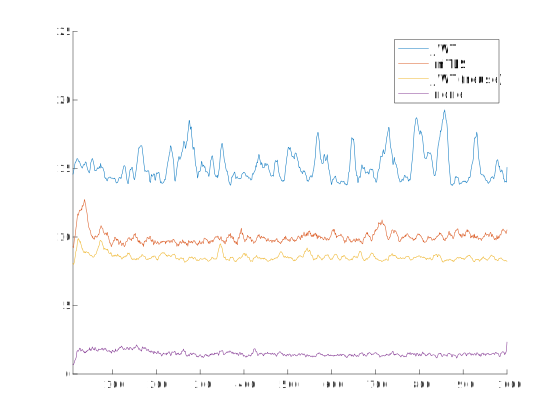
\includegraphics[trim=0 200 0 200, clip, width=\textwidth]{images/experiment/experiment-trend.pdf}
	\caption{Smoothened trend of the average request duration comparing the discussed authentication mechanisms excluding the first request}
	\label{fig:trend}
\end{figure}

\section{Conclusion}
This experiment compared the request durations of the two previously authentication mechanisms.
The results showed that the request durations between the mechanism using self-signed JWTs and mTLS are very similiar.
Depending on the implementation of the JWT approach it can consume up to ...\% more time or up to ...\% less time.
Therefore the performance is not the most crucial criterion when the two authentication mechanisms are compared since it's just a matter of milliseconds. 

Nevertheless for time critical projects in which each millisecond matters, self-signed JWTs are the better choice, since the performance can be optimized in multiple ways.
For example the certificates of the services can be distributed even before the first request is performed.
Or the validity timespan of the tokens can be increased so the same tokens can be used for a longer timespan.


\chapter{Final Remarks}
\label{cha:final_remarks}

\section{Discussion}
This thesis compared and explained the most popular mechanisms for mutual authentication in a microservice deployment.
Both mechanisms are based on public-key cryptography, but each mechanism has its own motivations and challenges.

Mutual TLS is an efficient and straightforward authentication mechanism.
The implementation of mTLS is very simple since the TLS protocol defines the processes.
Otherwise, mTLS does not provide many configuration parameters, and it does not allow to add custom functionalities, like sharing the user context without additional technologies.
Nevertheless, if a developer aims to implement only service-to-service authentication, mTLS is the preferred authentication mechanism.

As soon as nonrepudiation is required, self-signed JWTs are the superior authentication mechanism.
Furthermore, JWTs make identity propagation more convenient and allow the developers to customize the authentication mechanism and add additional parameters.
On the other hand, the implementation of self-signed JWTs is more challenging and requires each service to know how to work with JWTs.
Therefore choosing JWTs over mTLS would be unnecessary overhead when the target is implementing only service-to-service authentication.
The decision if the additional control of the approach using self-signed JWTs is worth the overhead has to be evaluated for each project independently.

The experiment of chapter~\ref{cha:experiment} showed that the performance of the compared authentication mechanisms is very similar.
According to the experiment results, the performance of the approach using self-signed JWTs is very dependent on the implementation of the mechanisms.
In some cases, using self-signed JWTs results in a lower request duration, but in some situations, it results in a higher request duration.
Therefore the performance is not a criterion that makes any mechanism superior to the other.

The biggest challenge of both authentication mechanisms is key management.
Both mechanisms require a PKI and require handling all associated key management tasks.
Therefore, implementing the authentication mechanisms is less challenging than key management.
Nevertheless, the level of security that is provided using public-key cryptography is worth the expenses.

\section{Summary}
Service-to-service authentication is a requirement caused by the migration to the microservice architecture.
Function calls within the monolithic backend migrate to remote calls.
Remote calls have to assure authentication, confidentiality, and integrity.
Confidentiality and integrity can be assured using TLS, but authentication of both parties requires additional mechanisms.

This thesis compared two of the most popular authentication mechanisms for service-to-service authentication.
Therefore the fundamentals and concepts of the compared authentication mechanisms were described in detail.
Additionally, a project using the discussed mechanisms was reviewed, and the consequences of the different mechanisms were described.
In the end, an experiment comparing the performance of the discussed authentication mechanisms was performed, and the results were discussed.


%% Is just a file for the listings of the presentation, because the LaTeX template does not provide a simple way to include code
\chapter{Listings}

\begin{CsCode}
	...
	var userManagement = new UserMangagement();
	User user = userManagement.getUser(userId);
	...
\end{CsCode}

\begin{CsCode}
	...
	var userClient = new UserMangagementClient("http://usermanagement.swapindo.com/", Program.httpClient);
	User user = userClient.UserAsync(userId)
		.GetAwaiter()
		.GetResult();
	...
\end{CsCode}

%\chapter{Implementation}
\label{cha:Implementation}
This chapter shows an implementation of the authentication mechanisms discussed in chapter~\ref{cha:authentication_mechanisms}.
The trust the network approach is not implemented in this chapter because it is deprecated and should not be used anymore. 

This implementation aims not to teach how to implement the discussed authentication mechanisms. It should help to gain a good understanding of how the mechanisms work.
Security critical features like service-to-service authentication are not recommended to be implemented and maintained by developers, which are not specialized for software security.
Therefore it is always good to use software as a platform applications like Kubernetes.
The most popular service mesh for Kubernetes is Istio.
It provides all security mechanisms, which are implemented in this chapter.
The implementation of Istio might differ from the following implementation, but the concepts stay the same.

\section{Implementation of mTLS}
This chapter shows the implementation of service-to-service authentication using mutual TLS. 
The following snippets are based on an ASP.NET 5.0 Web API written in C\# and the keys are generated using the cli\footnote{Command line interface} of OpenSSL.
Even if the implementation looks different in other languages, the code snippets should help understand the used mechanisms in more detail.

\subsection{Create Certificate Authority}
The following commands will create a key pair and a certificate for the CA.
The parameters of the following commands might vary, depending on how security-critical an application is.
The certificate of the CA is self-signed and does only include the subject field.
The CA has a 4096-bit RSA key, which does not mean that a 2048-bit key is not valid, but a 4096-bit key is much harder to brute force.
The key pair is also encrypted using the AES algorithm with a 256-bit key. Therefore anybody who has physical access to the file also needs a password to read the content.
The certificate of the CA is valid for one year, this period always depends on the application.
\begin{enumerate}
    \item Create key pair: \\ 
    \lstinline{openssl genrsa -aes256 -passout pass:"capassword" -out ca.key 4096}
    \item Create self-signed certificate: \\
    \lstinline{openssl req -new -passin pass:"capassword" -key ca.key -x509 -days 365} \\
    \lstinline{-out ca.crt -subj "/CN=ca.swapindo.com"}
\end{enumerate}

\subsection{Create key pair and a signed certificate for a service} \label{sec:createkeypair}
The following commands will create a key pair and a certificate for a service. 
The CA signed the certificate and is later used in the TLS handshake.
Each service has to do this process, therefore it is good to use automation tools like Netflix uses Lemur~\cite{dias2020microservices}.
The certificates of the services get a shorter lifetime of 30 days, this might also differ depending on how security-critical the application is. 
Additionally, a PFX file is created, it is an encrypted container that includes both the certificate and the key pair.
The PFX file is not required, but it makes it more convenient to parse the file from a C\# program.
\begin{enumerate}
    \item Create key pair: \\ 
    \lstinline{openssl genrsa -aes256 -passout pass:"servicepassword" -out service.key 4096}
    \item Create certificate signing request: \\
    \lstinline{openssl req -passin pass:"servicepassword" -new -key service.key} \\
    \lstinline{-out service.csr -subj "/CN=adservice.swapindo.com"}
    \item Sign certificate, using the private key of the CA: \\
    \lstinline{openssl x509 -req -passin pass:"capassword" -days 30 -in service.csr -CA ca.crt} \\
    \lstinline{-CAkey ca.key -set_serial -01 -out service.crt}
    \item Create PFX file, which is later used, to send HTTPS Requests: \\
    \lstinline{openssl pkcs12 -export -out service.pfx -passin pass:"servicepassword" -inkey} \\ 
    \lstinline{service.key -in service.crt -passout pass:"passwordService"}
\end{enumerate}

\subsection{Certificate validation logic}
The code of listing~\ref{lst:CertificateAuthority} shows an implementation of the validation logic, implemented in a static class, the \textit{CertificateAuthority}.
The \textit{CertificateAuthority} makes use of the singleton pattern, which is good practice since the validations do not store any state, and the file which holds the CA certificate should not be parsed at each request.
The validation is done using an \textit{X509Chain} of the dotnet cryptography library.
The chain is configured to ignore revocation because the revocation is beyond the scope of this implementation.
Furthermore, the chain is configured to use the \textit{CustomTrustStore}, because this is the place where the appended certificates are stored.

The \textit{AppendCertificate} function is used to append the certificate of the self-signed root CA to the \textit{CustomTrustStore} of the chain.
The CA certificate could also be appended in the constructor of the CA, but providing a function for this purpose makes the class more flexible since multiple CAs can be added, and the path of the certificate can vary between the applications.

The validation of the certificate is performed in the \textit{ValidateCertificate} function. 
It uses the \textit{Build} function of the \textit{X509Chain}, which returns true or false, whether the certificate is valid or not.
Using the cryptographic functionalities of popular libraries is always safer than implementing them by hand.

\noindent \begin{minipage}{\linewidth}
\begin{CsCode}[label={lst:CertificateAuthority}, caption={CertificateAuthority class, that is responsible for the certificate validation~\cite{impsingleton,impvalidatecert,impx509chain}},captionpos=b]
 public class CertificateAuthority {
    private static X509Chain chain = null;
    private static CertificateAuthority instance = new CertificateAuthority();
    public static CertificateAuthority Instance { get { return instance; } }
    
    static CertificateAuthority() {
        // Create chain
        chain = new X509Chain();
        
        // Set options
        chain.ChainPolicy.RevocationMode = X509RevocationMode.NoCheck;
        chain.ChainPolicy.TrustMode = X509ChainTrustMode.CustomRootTrust;
    }
    
    public void AppendCertificate(X509Certificate cert) {
        // Add the certificate to the custom trust store
        chain.ChainPolicy.CustomTrustStore.Add(cert);
    }
    
    public bool Validate(X509Certificate2 cert) {
        try {
            return chain.Build(cert);
        } catch (Exception ex) {
            return false;
        }
    }
}
\end{CsCode}
\end{minipage}

\subsection{Service configuration}
The server, which hosts the application has to be configured to allow the client to send certificates. 
This process may vary, depending on the used technologies.
The code in listing~\ref{lst:ConfigureKestrel} shows how this is done using the Kestrel web server.
This only allows the clients to send certificates, but it does not validate them against the CA.
Therefore every request, which uses a valid certificate is considered valid, even if the certificate is signed by an unknown CA.

\noindent \begin{minipage}{\linewidth}
\begin{CsCode}[label={lst:ConfigureKestrel}, caption={Configure Kestrel to allow certificates~\cite{implkritnermtls}},captionpos=b]
webBuilder.ConfigureKestrel(kestrelOptions => {
    kestrelOptions.ConfigureHttpsDefaults(httpOptions => {
        httpOptions.ClientCertificateMode = ClientCertificateMode.AllowCertificate;
    });
});
\end{CsCode}
\end{minipage}

Listing~\ref{lst:ConfigureService} shows how the services are configured to verify that the incoming certificate is signed by the trusted root CA.
The validation is configured to neglect the revocation and allow only chained certificates. Otherwise, somebody could use the key pair of the CA itself to access the service.
If the certificate is considered valid, it is additionally checked by the \textit{CertificateAuthority}, which was shown in listing~\ref{lst:CertificateAuthority}.
If the client's certificate is valid and is signed by the CA, the client is authenticated and is allowed to access the functionalities of the service.

\noindent \begin{minipage}{\linewidth}
\begin{CsCode}[label={lst:ConfigureService}, caption={Configure the certificate authentication for the service~\cite{implkritnermtls}},captionpos=b]
services.AddAuthentication(CertificateAuthenticationDefaults.AuthenticationScheme)
.AddCertificate(options => {
    options.AllowedCertificateTypes = CertificateTypes.Chained;
    options.RevocationMode = X509RevocationMode.NoCheck;
    options.Events = new CertificateAuthenticationEvents() {
        OnCertificateValidated = context => {
            if (CertificateAuthority.Instance.Validate(context.ClientCertificate)) {
                context.Success();
            } else {
                context.Fail("Certificate validation failed");
            }
            return Task.CompletedTask;
        },
        OnAuthenticationFailed = context => {
            context.Fail("Certificate validation failed");
            return Task.CompletedTask;
        }
    };
});
\end{CsCode}
\end{minipage}

The code of listing~\ref{lst:ConfigureService} shows how to configure the client authentication for the service.
But the service has to be configured to use the implemented authentication mechanism.
Therefore the statement \lstinline{app.UseAuthentication();} has to be added to the \textit{Configure} function of the \textit{Startup} class. 
Since the service was configured to allow certificates and not to require them. 
The API functions can define whether a client needs a valid certificate or not.
This is done by appending the \lstinline{[Authorize]} annotation before the function declaration.
The code of listing~\ref{lst:ConfigureKestrel} can be adopted to require certificates, which would not allow any access to the API without a valid certificate.

\subsection{Use the certificate for requests}
Since the services consume the functionalities of other services, they have to be configured to use client certificates for their request.
The creation of a client certificate was shown in section~\ref{sec:createkeypair}.
Listing~\ref{lst:ConfigureHttpClient} shows how the client certificate is appended to a \textit{HttpClient}, which is later injected into the services, using dependency injection.
It is not required to use dependency injection for the HttpClient, but it is good practice to use it according to the documentation.
A considerable advantage of the dependency injection is that the pfx file does not have to be parsed for each request.
Instead, it is parsed once and injected into the controller when initialized.
The controller can then use the \textit{HttpClient} and perform requests without dealing with the client certificate.

\noindent \begin{minipage}{\linewidth}
\begin{CsCode}[label={lst:ConfigureHttpClient}, caption={Append Certificate to HttpClient~\cite{implclientfactory, implconfighandler}},captionpos=b]
services.AddHttpClient("mtlsclient")
.ConfigurePrimaryHttpMessageHandler(() => {
    HttpClientHandler handler = new HttpClientHandler();
    handler.ClientCertificates
        .Add(new X509Certificate2(@"service.pfx", "passwordService"));
    return handler;
});
\end{CsCode}
\end{minipage}

%Listing~\ref{lst:UseHttpClient} shows how the configured HttpClient is injected into a Controller and then used to perform a request.
%
%\noindent \begin{minipage}{\linewidth}
%\begin{CsCode}[label={lst:UseHttpClient}, caption={Use the injected HttpClient~\cite{impluseclient}},captionpos=b]
%[ApiController]
%public class ForwardUsersController : ControllerBase {
%    private HttpClient httpClient;
%
%    public ForwardUsersController(IHttpClientFactory factory) {
%        httpClient = factory.CreateClient("mtlsclient");
%    }
%
%    [HttpGet]
%    public async Task<string> Get() {
%        using (var response = await httpClient.GetAsync(apiUrl)) {
%            // process response
%        }
%    }
%}
%\end{CsCode}
%\end{minipage}

%%%-----------------------------------------------------------------------------
\appendix                                                             % Appendix 
%%%-----------------------------------------------------------------------------

%\chapter{Technical Details}
\label{app:TechnicalDetails}

%\section{JSON Web Token Registered Claims}
%\begin{table}[H]
%    \centering
%    \begin{tabular}{|l|l|p{7cm}|}
%    \hline
%        \textbf{Claim Identifier} & \textbf{Name} & \textbf{Content} \\
%    \hline
%        iss & Issuer & identifies the principle, that issued the JWT \\
%    \hline
%        sub & Subject & identifies the principle that is the subject of the JWT \\
%    \hline 
%        aud & Audience & identifies the principle that the JWT is intended for \\ 
%    \hline
%        exp & Expiration Time & identifies the expiration time on or after which the JWT must not be accepted for processing \\
%     \hline
%        nbf & Not Before & identifies the time before which the JWT must not be accepted for processing \\
%    \hline
%        ist & Issued At & identifies the time at which the JWT was issued \\
%    \hline
%        jti & JWT ID & provides a unique identifier for the JWT \\
%    \hline
%    \end{tabular}
%    \caption{JWT Registered Claims~\cite{jwtrfc}}
%    \label{tab:jwt_registered claims}
%\end{table}
 % Technical supplements

%%%-----------------------------------------------------------------------------
\backmatter                           % Back part (bibliography, glossary, etc.)
%%%-----------------------------------------------------------------------------

\MakeBibliography % References

%%%-----------------------------------------------------------------------------
% Special page for checking print size
%%%-----------------------------------------------------------------------------

%\include{back/printbox}

%%%-----------------------------------------------------------------------------
\end{document}
%%%-----------------------------------------------------------------------------
